% ============================================================
%  Stable Causal Targeting with Machine Learning
%  17-minute talk, Beamer (Metropolis)
%  Based on: new submission/jbes_submission_marked.tex
%  Background: Dwivedi et al. (2020), StaDISC + PCS framework
%  Compile:  xelatex talk.tex  (run twice)
% ============================================================
\documentclass[aspectratio=169,11pt]{beamer}

% ---------- Theme ----------
\usetheme[progressbar=frametitle,
         numbering=fraction,
         sectionpage=progressbar,
         subsectionpage=progressbar,
         block=fill]{metropolis}

\usepackage{appendixnumberbeamer}
\usepackage{booktabs}
\usepackage{array}
\usepackage{amsmath,amssymb}
\usepackage{bm}
\usepackage{xcolor}
\usepackage{graphicx}
\usepackage{tikz}
\usetikzlibrary{positioning, arrows.meta, calc, fit, shapes.geometric}

\graphicspath{{figs/}}

% ---------- Fonts (Metropolis prefers Fira Sans; load by filename) ----------
\usepackage{iftex}
\ifxetex
  \usepackage{fontspec}
  \IfFontExistsTF{FiraSans-Light.otf}{%
    \setsansfont{FiraSans-Light.otf}[
      BoldFont       = FiraSans-Medium.otf,
      ItalicFont     = FiraSans-LightItalic.otf,
      BoldItalicFont = FiraSans-MediumItalic.otf]
    \setmonofont{FiraMono-Regular.otf}[BoldFont=FiraMono-Medium.otf]
  }{}
\fi

% ---------- Colors ----------
\definecolor{accent}{HTML}{2A6F97}
\definecolor{accentdark}{HTML}{013A63}
\definecolor{warm}{HTML}{C75B12}
\definecolor{softgray}{HTML}{6B7280}

\setbeamercolor{progress bar}{fg=accent}
\setbeamercolor{frametitle}{bg=accentdark, fg=white}
\setbeamercolor{title separator}{fg=accent}
\setbeamercolor{alerted text}{fg=warm}
\setbeamercolor{section in toc}{fg=accentdark}
\setbeamercolor{block title}{bg=accent!15, fg=accentdark}
\setbeamercolor{block body}{bg=accent!5}

\setbeamersize{text margin left=10mm, text margin right=10mm}
\setbeamertemplate{navigation symbols}{}

% Tighten list spacing so dense frames fit Fira's metrics
\setlength{\parskip}{0.2em}
\makeatletter
\def\@listi{\leftmargin\leftmargini
           \topsep    4\p@ \@plus2\p@ \@minus2\p@
           \parsep    0\p@
           \itemsep   2\p@ \@plus1\p@}
\makeatother

% ---------- Convenience macros ----------
\newcommand{\rsquare}{\ensuremath{\mathcal{R}^2_{\mathrm{C}}}}
\newcommand{\CalSlope}{\ensuremath{\operatorname{CalSlope}}}
\newcommand{\MeanDeltaTopTen}{\ensuremath{\overline{\Delta}_{0.10}}}
\newcommand{\het}{\textcolor{accent}{\textbf{heterogeneous}}}
\newcommand{\noisy}{\textcolor{warm}{\textbf{noisy}}}

% ---------- Title metadata ----------
\title{Stable Causal Targeting with Machine Learning}
\subtitle{Application to a Behavioral Field Experiment in Consumer Finance}
\author{Zhen Zhong\inst{1} \and Junni Zhang\inst{2}}
\institute{\inst{1}TCL Corporate Research \and \inst{2}Peking University}
\date{}

\begin{document}

\maketitle

% ============================================================
\begin{frame}{Motivation: experiments estimate averages, but responses vary}
\begin{itemize}
  \item Firms run randomized field experiments to estimate \alert{average treatment effects} (ATE).
  \item But responses are often \het, and in behavioral settings also \noisy.
  \item Flexible ML estimators of CATEs can \alert{overfit} training folds, show \alert{weak calibration} on new data, and yield \alert{unstable} prioritization rules.
  \item Aggressive subgroup search without adjustment finds effects that do \textbf{not} replicate.
\end{itemize}

\vspace{0.2em}
\begin{block}{Goal}
A practical, stability-first workflow for subgroup targeting that survives repeated data perturbations and an untouched holdout.
\end{block}
\end{frame}

% ============================================================
\begin{frame}{Background: StaDISC and the PCS framework}
\textbf{StaDISC} — \emph{Stable Discovery of Interpretable Subgroups via Calibration} \small(Dwivedi et al., 2020)\normalsize
\begin{itemize}
  \item Originally built for subgroup discovery in \alert{clinical trials}.
  \item True CATE unobserved $\Rightarrow$ cannot use AUC; use \alert{calibration} instead.
  \item Bin units by CATE estimates; compare bin-mean CATE vs.\ difference-in-means.
\end{itemize}

\vspace{0.1em}
\textbf{PCS framework} — \emph{Predictability, Computability, Stability} \small(Yu \& Kumbier, 2018, 2020)\normalsize:
\textbf{P}redictability $=$ out-of-sample accuracy; \textbf{C}omputability $=$ feasible \& reproducible; \textbf{S}tability $=$ robust to perturbations in data, model, and sampling.

\vspace{0.15em}
\begin{alertblock}{This paper}
Extend StaDISC from clinical trials to a \alert{consumer-banking} field experiment with smaller effects and noisier outcomes.
\end{alertblock}
\end{frame}

% ============================================================
\begin{frame}{What we add to StaDISC}
\begin{itemize}
  \item \textbf{Setting:} behavioral finance (low signal-to-noise) instead of clinical trials.
  \item \textbf{Feature selection:} Lasso pre-screening (519 $\to$ 14 features) — not in original StaDISC.
  \item \textbf{Selection rule:} replace the $t$-statistic grid with a \alert{calibration-slope nested-ensemble path}:
    \begin{enumerate}
      \item order candidate estimators by validation-fold \CalSlope,
      \item build nested equal-weight mean ensembles along that order,
      \item pick the ensemble maximizing the top-10\% targeting contrast \MeanDeltaTopTen.
    \end{enumerate}
  \item \textbf{Validation:} evaluate the selected ensemble on a completely untouched holdout.
\end{itemize}
\end{frame}

% ============================================================
\section{The YK overdraft experiment}

\begin{frame}{Setting: unshrouding overdraft costs in Turkey}
\textbf{Alan, Cemalcular, Karlan \& Zinman (2018)} — Yapi Kredi (YK), one of Turkey's largest banks. 108{,}000 marginal overdrafters randomized to text-message arms; outcome $=$ overdraft usage.

\vspace{0.2em}
\begin{itemize}
  \item \textbf{Availability reminder} $\Rightarrow$ \emph{increased} usage (makes overdraft salient).
  \item \textbf{Discount message} (50\% off 60\% APR) $\Rightarrow$ \emph{decreased} usage (unshrouds the cost).
  \item \textbf{Bundled messages} (discount $+$ bill-payment / debit-card) $\Rightarrow$ \emph{further} decrease.
\end{itemize}

\vspace{0.2em}
\textbf{Shrouded-attributes logic} (Gabaix \& Laibson, 2006): unshrouding may produce \het\ responses —
\begin{itemize}
  \item \emph{financially sophisticated} consumers already aware of overdraft,
  \item \emph{liquidity-constrained} consumers with acute short-term needs.
\end{itemize}
\end{frame}

% ============================================================
\begin{frame}{Data and sample design}
\textbf{Main comparison:} bill-payment bundled message vs.\ baseline availability reminder.

\vspace{0.5em}
\begin{columns}[T,onlytextwidth]
\column{0.5\textwidth}
\begin{itemize}
  \item Full sample: \textbf{36{,}024} customers
    \begin{itemize}
      \item 17{,}981 treated (bundled)
      \item 18{,}043 control (reminder)
    \end{itemize}
  \item Outcome: binary overdraft usage.
  \item Full-sample ATE $= -0.0138$ \;(SE 0.0049).
\end{itemize}

\column{0.5\textwidth}
\textbf{Split (stratified by treatment):}
\begin{itemize}
  \item \textbf{20\% holdout} — 7{,}205 customers; touched only at the very end.
  \item \textbf{80\% train/val} — 28{,}819 customers.
\end{itemize}

\vspace{0.4em}
\textbf{Cross-validation:} three stratified 4-fold splits \\
($\mathrm{cv}_{\mathrm{orig}}, \mathrm{cv}_0, \mathrm{cv}_1$) $\Rightarrow$ \alert{12 training-validation fold pairs}.
\end{columns}
\end{frame}

% ============================================================
\begin{frame}{Feature engineering \& selection}
\begin{itemize}
  \item Covariates: strata, reminder frequency, campaign type, prior activations, assets, deposits, debt, balances, credit-card usage, \dots
  \item Missing values $\Rightarrow$ missingness dummies $+$ zero imputation $\Rightarrow$ \textbf{519 features}.
  \item \textbf{Lasso selection} (treated / control separately, standardized): top-10 by $|\text{coef}|$ each $\Rightarrow$ union $=$ \alert{14 features} — \alert{extends} StaDISC.
\end{itemize}

\begin{figure}
\centering

\includegraphics[width=0.40\textwidth]{fausebal_lasso_coef.png}
\end{figure}
\end{frame}

% ============================================================
\section{CATE models \& calibration check}

\begin{frame}{23 CATE estimation models}
\small
\begin{tabular}{p{2.6cm} p{9.5cm} l}
\toprule
\textbf{Family} & \textbf{Idea} & \textbf{\#} \\
\midrule
S-learner & One model on $(X,Z)$; CATE $=\hat\mu(x,1)-\hat\mu(x,0)$ & 2 \\
T-learner & Separate $\hat\mu_1,\hat\mu_0$; CATE $=\hat\mu_1-\hat\mu_0$ & 4 \\
X-learner & Impute ITEs, then regress (K\"unzel et al., 2019) & 4 \\
R-learner & Residualize $Y,Z$ on $X$, then weighted regression (Nie \& Wager, 2021) & 9 \\
Causal tree / forest & Honest partitions / ensembles (Athey \& Imbens; Wager \& Athey) & 4 \\
\midrule
\multicolumn{2}{r}{\textbf{Total}} & \textbf{23} \\
\bottomrule
\end{tabular}

\vspace{0.5em}
\normalsize
Base learners: \texttt{Lasso}, penalized logistic, \texttt{RF}, \texttt{XGB}. \\
Hyperparameters tuned by 4-fold CV on $\mathrm{cv}_{\mathrm{orig}}$ (200 random configs each); fixed on $\mathrm{cv}_0,\mathrm{cv}_1$.
\end{frame}

% ============================================================
\begin{frame}{Calibration-based reality check ($\rsquare$)}
True CATE $\tau(x_i)$ is unobserved $\Rightarrow$ AUC is not available. Use \alert{calibration}.

\vspace{0.4em}
\textbf{Key identity} for any subgroup $G$ of the feature space:
\[
\mathbb{E}[Y(1)-Y(0)\mid X\in G] \;=\; \mathbb{E}\!\left[\tau(X)\mid X\in G\right].
\]

\vspace{0.2em}
\begin{itemize}
  \item Bin units by CATE estimates into 10 deciles $\mathcal{G}_1,\dots,\mathcal{G}_{10}$.
  \item In each bin compare \alert{mean model CATE} $\bar{\mathfrak{M}}$ vs.\ \alert{difference-in-means} $\hat\tau$.
\end{itemize}

\vspace{0.2em}
\textbf{Cal-Score} $= \sum_j \tfrac{|\mathcal{G}_j\cap\mathcal{S}|}{|\mathcal{S}|}\,\bigl|\bar{\mathfrak{M}}_{\mathcal{G}_j\cap\mathcal{S}} - \hat\tau_{\mathcal{G}_j\cap\mathcal{S}}\bigr|,\quad
\rsquare = 1 - \dfrac{\text{Cal-Score}(\mathfrak{M})}{\text{Cal-Score}(\hat\tau_{\mathrm{ATE}})}.$

\vspace{0.2em}
$\rsquare\!\to\!1$ good calibration; $\rsquare\!\le\!0$ no better than a constant ATE $\Rightarrow$ overfitting.
\end{frame}

% ============================================================
\begin{frame}{Result: poor global calibration $=$ overfitting}
\begin{columns}[T,onlytextwidth]
\column{0.52\textwidth}

\includegraphics[width=\textwidth]{fausebal_r2_distribution.png}

\column{0.48\textwidth}
\begin{itemize}
  \item Training $\rsquare$: mean $0.30$, median $0.28$.
  \item Validation $\rsquare$: mean $-0.21$, median $-0.13$.
  \item Systematic gap $=$ \alert{models fit noise}, not real heterogeneity.
  \item Echoes the original StaDISC finding on clinical data.
\end{itemize}

\vspace{0.4em}
\textbf{Bottom line:} \emph{globally}, all 23 CATE models fail to calibrate on held-out folds.
\end{columns}
\end{frame}

% ============================================================
\begin{frame}{Calibration plots: reasonable in-sample, breaks out-of-sample}
\begin{figure}
\centering

\includegraphics[width=0.78\textwidth]{fausebal_calibration_plot.png}
\end{figure}
\vspace{-0.4em}
\small
\texttt{x\_rf} (X-learner$+$RF) and \texttt{r\_rflasso} (R-learner, RF$\to$Lasso). Triangles $=$ model CATE; circles $=$ difference-in-means $\pm 1$ SE. Left: training; Right: validation. Dashed $=$ overall ATE ($-0.0158$).
\end{frame}

% ============================================================
\begin{frame}{Quantile-based top subgroups: look for \emph{local} signal}
Global calibration fails, but a model may still \alert{rank} the top units correctly.

\vspace{0.2em}
For quantile $q\in\{0.9,0.8,0.7,0.6,0.5\}$ define the \alert{top subgroup} $\widetilde{\mathcal{G}}_q^{\,c}$ and the indicator
\[
B_q = \mathbf{1}\!\left\{\hat\tau_{\widetilde{\mathcal{G}}_q\cap\mathcal{S}_{\mathrm{VF}}} \;\le\; \hat\tau_{\widetilde{\mathcal{G}}_q^{\,c}\cap\mathcal{S}_{\mathrm{VF}}}\right\},\qquad
\bar B_q = \tfrac{1}{12}\sum_{f=1}^{12} B_q.
\]

\vspace{0.1em}
\begin{figure}
\centering

\includegraphics[width=0.42\textwidth]{fausebal_all_estimators.png}
\end{figure}
\vspace{-0.4em}
\small
Most models are poorly calibrated \emph{and} unstable; $q=0.9$ is the best-behaved $\Rightarrow$ focus on the \alert{top 10\%}.
\end{frame}

% ============================================================
\section{Selection \& validation}

\begin{frame}{Selection rule: a calibration-slope nested-ensemble path}
\textbf{Step 1 — Order by $\CalSlope$.} Cut training-fold CATE into 5 strata; regress observed stratum ATE $\hat\theta_{mfk}$ on mean predicted CATE $\bar\mu_{mfk}$, take the OLS slope $\CalSlope_{mf}=\hat\beta_{mf}$, average over folds: $\CalSlope_m=\tfrac{1}{|\mathcal F_m|}\sum_f\CalSlope_{mf}$. Order estimators from largest to smallest $\CalSlope_m$.

\vspace{0.15em}
\textbf{Step 2 — Nested mean ensembles.} Ensemble 1 $=$ top estimator; ensemble 2 $=$ top 2; \dots

\vspace{0.1em}
\textbf{Step 3 — Pick by top-10\% contrast.} For ensemble $e$, fold $f$:
\[
\Delta_{ef,0.10}=\hat\tau(\mathcal{G}_{ef}^{0.10})-\hat\tau(\mathcal{R}_{ef}^{0.10}),\qquad
\MeanDeltaTopTen(e)=\tfrac{1}{|\mathcal{F}_e|}\sum_{f}\Delta_{ef,0.10}.
\]
Select the ensemble with the \alert{largest $\MeanDeltaTopTen$} (ties $\Rightarrow$ fewer members). \small Public rule: $\CalSlope$ to order, $\MeanDeltaTopTen$ to select.
\end{frame}

% ============================================================
\begin{frame}{Selected ensemble on the YK data}
\begin{columns}[T,onlytextwidth]
\column{0.46\textwidth}
\begin{table}
\centering
\small
\begin{tabular}{@{}lc@{}}
\toprule
& \textbf{Value} \\
\midrule
Ordering statistic & $\CalSlope$ \\
Candidate path & nested ensembles \\
Selection statistic & $\MeanDeltaTopTen$ \\
\midrule
\textbf{Selected (2 of 23)} & \\
\quad \texttt{x\_rf} & \checkmark \\
\quad \texttt{r\_rflasso} & \checkmark \\
\midrule
Targeting quantile & top 10\% \\
\bottomrule
\end{tabular}
\end{table}

\column{0.54\textwidth}
\begin{itemize}
  \item Despite negative full-sample ATE, the top-10\% subgroup shows a \alert{positive} effect.
  \item Two very different families (X-learner, R-learner) agree $\Rightarrow$ stability signal.
  \item The ensemble is small (2 members), reducing overfitting risk vs.\ larger blends.
\end{itemize}
\end{columns}
\end{frame}

% ============================================================
\begin{frame}{Final validation on the untouched holdout}
\begin{table}
\centering
\begin{tabular}{@{}lcc@{}}
\toprule
& \textbf{Train-Val} & \textbf{Holdout} \\
\midrule
Total sample size & 28{,}819 & 7{,}205 \\
Top-10\% subgroup size & 2{,}882 & 723 \\
Subgroup ATE (SE) & 0.0407 (0.0175) & \alert{0.0617 (0.0346)} \\
$t$-statistic & 2.32 & 1.78 \\
95\% CI & [0.0064, 0.0750] & [$-$0.0061, 0.1296] \\
90\% CI & [0.0119, 0.0695] & \alert{[0.0048, 0.1187]} \\
\bottomrule
\end{tabular}
\end{table}

\vspace{0.5em}
\begin{itemize}
  \item Holdout top-10\% ATE $= +6.17$ pp, \alert{significant at the 10\% one-sided level}.
  \item Effect \emph{grows} from train-val to holdout $\Rightarrow$ not an in-sample artifact.
  \item Full-sample ATE was $-1.38$ pp: targeting flips the sign for the right subgroup.
\end{itemize}
\end{frame}

% ============================================================
\begin{frame}{The other two arms do \alert{not} replicate}
Same procedure applied to the other treatment-arm comparisons:

\vspace{0.3em}
\begin{table}
\centering
\small
\begin{tabular}{@{}p{0.34\textwidth} p{0.34\textwidth} c@{}}
\toprule
\textbf{Treatment arm} & \textbf{Selected ensemble} & \textbf{Holdout ATE (SE), $t$} \\
\midrule
Debit-card bundled msg & \texttt{s\_rf} & $-0.0724$ (0.0362), $-2.00$ \\
Availability reminder vs.\ none & \shortstack[l]{\texttt{x\_rf|x\_lasso}\\\texttt{|t\_lasso|x\_logistic}} & $-0.0119$ (0.0306), $-0.39$ \\
\bottomrule
\end{tabular}
\end{table}

\vspace{0.3em}
\begin{itemize}
  \item Neither produces a positive holdout effect.
  \item The \alert{bill-payment bundled message} is the only arm with a positive top-10\% holdout signal.
  \item Stability screening prevents overconfident targeting recommendations.
\end{itemize}
\end{frame}

% ============================================================
\begin{frame}{Simulation: $\MeanDeltaTopTen$ picks a near-best ensemble}
\begin{figure}
\centering
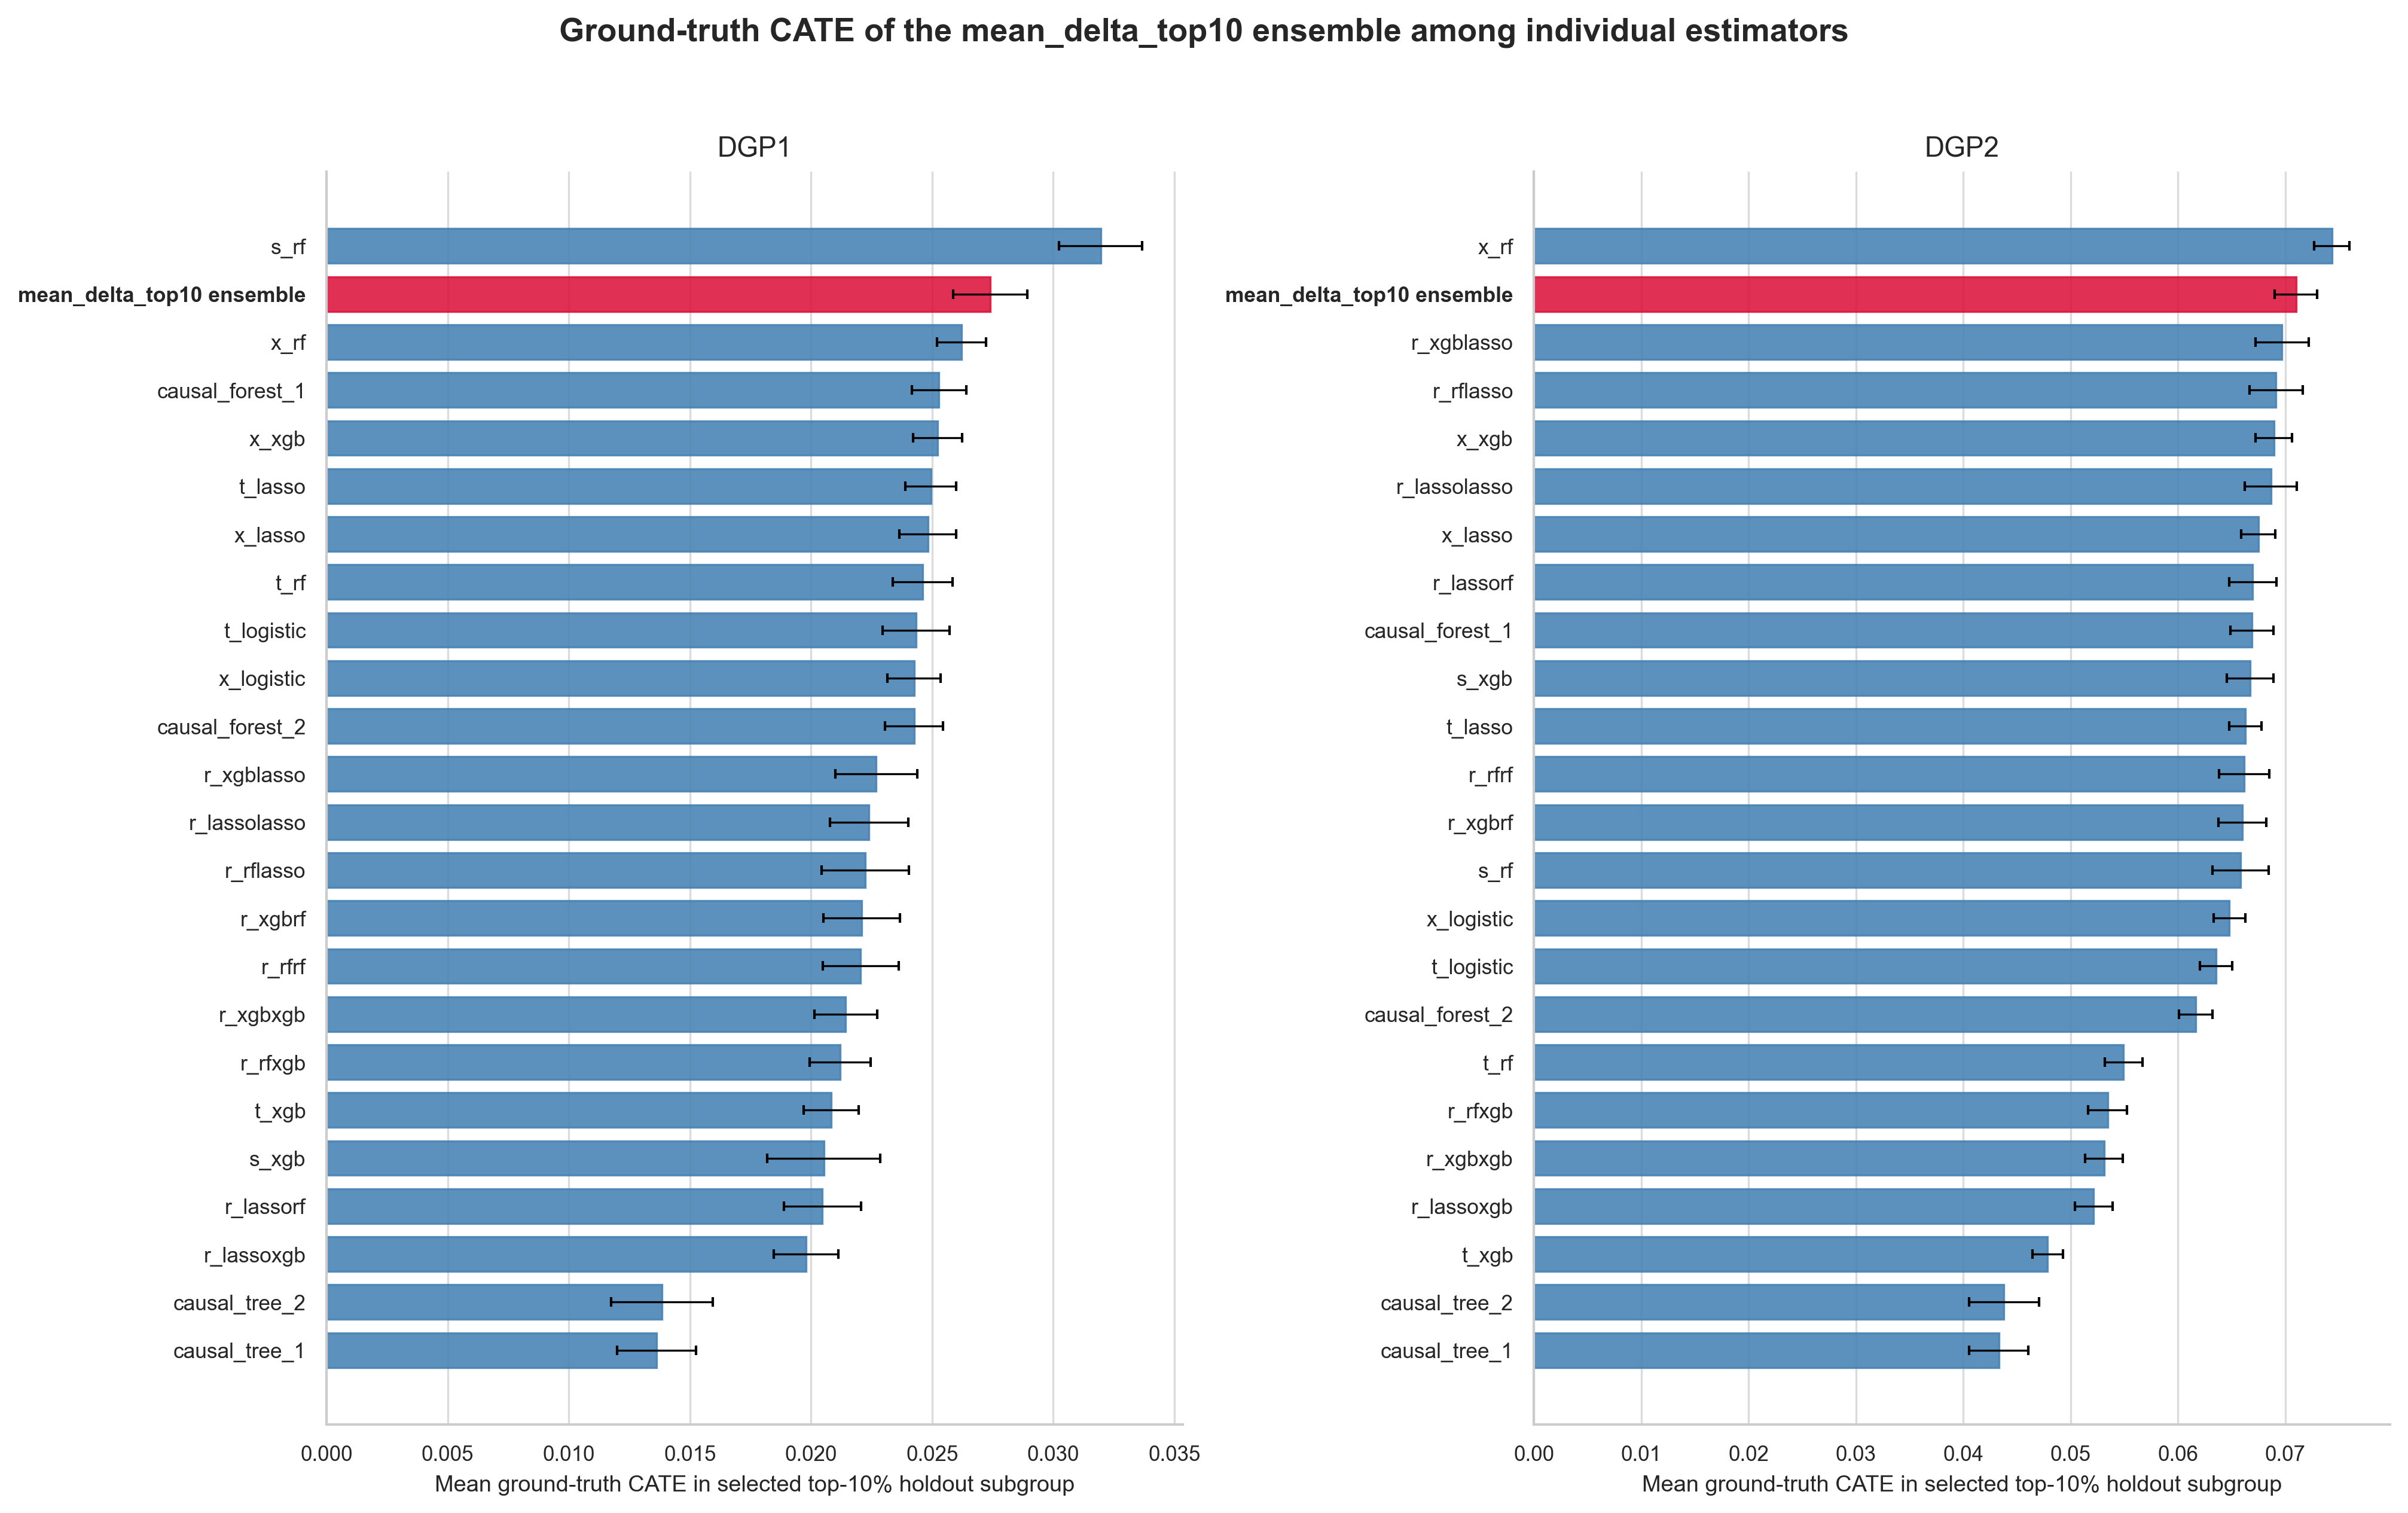
\includegraphics[width=0.54\textwidth]{mc_true_cate_top10_mean_delta_top10_ensemble_vs_estimators.png}
\end{figure}
\vspace{-0.3em}
\small
Ground-truth top-10\% CATE of the ensemble selected by \MeanDeltaTopTen\ vs.\ all 23 individual estimators, across two simulation DGPs. The selected ensemble attains true-CATE rank $\le 2$ in both designs.
\end{frame}

% ============================================================
\section{Conclusion}

\begin{frame}{Takeaways}
\begin{itemize}
  \item In low-signal behavioral experiments, \alert{global CATE estimation fails}: all 23 models are poorly calibrated out-of-sample.
  \item Yet a \alert{calibration-slope nested-ensemble} rule identifies a top-10\% subgroup with a \alert{positive holdout effect} ($+6.17$ pp, $p<0.10$ one-sided).
  \item The rule is public and simple: $\CalSlope$ to order, $\MeanDeltaTopTen$ to select.
  \item Other arms do not replicate $\Rightarrow$ stability screening prevents overconfident targeting.
\end{itemize}

\vspace{0.3em}
\begin{block}{PCS as a template}
Smaller effects and noisier outcomes than the original clinical-trial StaDISC — yet calibration reality checks, validation-fold selection, and a quantile-based top subgroup still deliver a useful targeting rule.
\end{block}
\end{frame}

% ============================================================
\begin{frame}[standout]
Thank you \\[0.3em]
\normalsize Questions \& discussion welcome
\end{frame}

\end{document}
